We use 3 augmentations: a random horizontal flip; a random perspective change; and a random brightness jitter; all of which preserve a patch's class (see Figure \ref{fig:Q1_4}).
The horizontal flip and random perspective change, help the model better generalize spatially.
The brightness jitter aims to instill a brightness invariance in our model, helping tackle the night vs day issue.
Although a brightness standardization may have been better.

To makes patches a constant size we scale, preserving aspect ratio, and then pad.
We found this gave better results than scaling without preserving aspect ratio.

\begin{figure}[h!]
  \begin{center}
  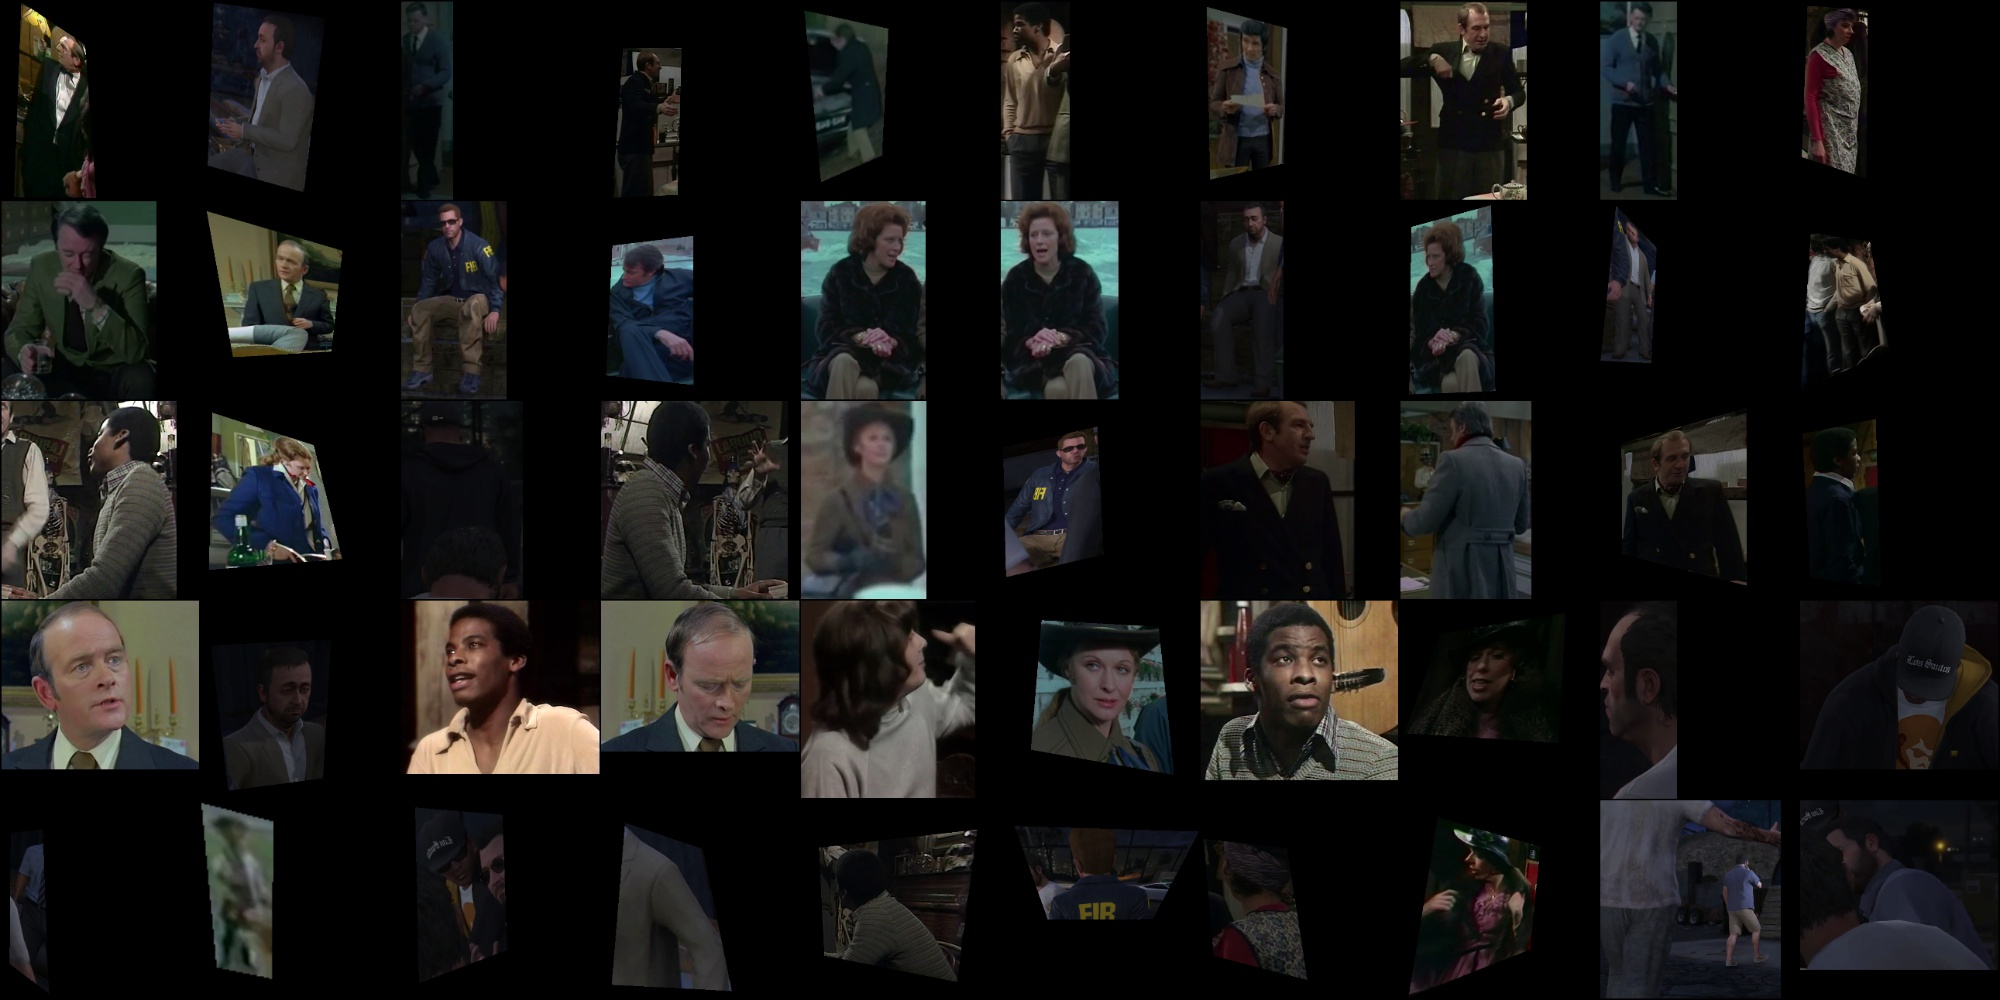
\includegraphics[scale=0.2]{Q1_4_patches.jpg}
    \caption{Q1.4 sample of augmented human patches.}
    \label{fig:Q1_4}
  \end{center}
  \end{figure}